\documentclass[a4paper, 10pt, notitlepage, twocolumn]{article}

\usepackage{ucs}
\usepackage[utf8]{inputenc}
\usepackage{amsmath}
\usepackage{amsfonts}
\usepackage{amssymb}
\usepackage[english]{babel}
\usepackage[justification=centering]{caption}
\usepackage{fontenc}
\usepackage{graphicx}
\usepackage{listings}
\usepackage{placeins}
\usepackage{tikz}

\usepackage[a4paper, colorlinks]{hyperref}

\author{Simon R. Klaver}
\title{A weighty research into Deep Learning}

\begin{document}
\maketitle

\tableofcontents

 \section{Introduction}
 \label{introduction}
  ``Deep Learning is the future!". This has undoubtly been said at some time by someone. But following the successes of AlphaGo $\cite{AlphaGo}$,  Deep Learning $\cite{DeepLearning}$ has been placed on the minds of many and is tested on new boundaries. For example,  the company behind AlphaGo,  called DeepMind,  has collaborated with game developer Blizzard to apply Deep Learning to StarCraft II,  a real-time strategy videogame $\cite{StarCraft}$. Compared to more conventional methods of machine learning,  which revolve around putting man-made algorithms to the test on problems,  this method relies on (controlled) randomness and,  at least seemingly,  uncontrolled computer logic. Is a self-conscious AI at hand? Perhaps. But in this paper,  we will focus on the weight patterns in the initialisation of a Deep Learning network. As Deep Learning networks seem to work better with more random variables and less human interaction $\cite{AlphaGoZero}$,  it may prove useful to focus on the parts that are still manipulated,  or manipulatable,  by mankind.\\
  In this paper we will first explain what a Deep Learning network is. Second we will explain our coding,  as that explains how the scope of this paper came to be. Then we will talk about our experiments,  and continue with the results of said experiments. In the last section we will conclude the paper and discuss possible future work.
  
 \section{What is a Deep Learning network?}
 \label{what}
    A network is,  in the most basic form,  a way to describe the relations between multiple entities. In this case,  this description means that there are multiple so-called ``nodes" as entities which have directed ``edges" as relations between them. Each of these nodes holds a floating point value,  just as the edges do. The values on the edges are called ``weights". The nodes are organised in rows (or columns,  depending on your representation),  where the outer row on one end is used to ``feed" the input to the network,  and the outer row on the other end is read to collect the output of the network. Between each of these rows,  there are edges connecting each node of the ``previous" row to every node in the ``next" row: however,  in case ``bias nodes" are used,  there will be no connections from the previous layer to a bias node. A bias node is a node which has a constant value,  for example -1. Therefore,  as long as the values on the edges are assured to be between 0 and 1,  the bias node ensures that if the other nodes in the same layer all have value 0,  the nodes in the next layer will not get the value 0. The weights of the edges are enforced to be between 0 and 1 by using a sigmoid function. A sigmoid is a curved function which approaches 0 for values below a certain treshold value $y$,  and approaches 1 for values above this treshold. The sigmoid used in our research is $g(x) = \frac{1}{1 + e^{-x}}$,  for which the forementioned number $y$ is 0. See Figure \ref{sigmoid} for a graph of this function. If $x$ is equal to 0,  $g(x)$ returns $\frac{1}{2}$. As for an example of such a network,  see Figure \ref{networkexample}; this network has three rows,  or ``layers",  and no bias nodes. In this paper we will only use networks with one hidden layer,  meaning that while using the algorithm of a Deep Learning network,  no actual ``deep" learning network is used.\\
    \begin{figure}
       \centering
       \includegraphics[width=.45\textwidth]{sigmoid}
       \caption{Graph of the sigmoid function\\$g(x) = \frac{1}{1 + e^{-x}}$.}
       \label{sigmoid}
    \end{figure}
    The network is ``trained",  or ``learns",  by ``backpropagation'',  which works as follows. First,  input is given in the input nodes and propagated through the network to the output node. The value in each node is the sum of the values of the nodes in the previous layer multiplied by the weights of the edges connecting the corresponding nodes in the previous layer to the current node. So if node $a$ connects to node $x$ with edge $b$,  and node $c$ connects to node $x$ with edge $d$,  then the value of node $x$ becomes the values of $a * b + c * d$. This process is repeated for each layer,  until all nodes in the output layer are assigned a value. Then the output can be compared to the expected output,  giving an error value. This error is for this paper the expected output minus the calculated output. Note that we will refer to both ``original output" and ``calculated output": the first is the value in the output node(s) at the end of the forward propagation,  the second is this value / these values but with the sigmoid applied to them. With this we can calculate the ``delta" value of each node. Assume the network in Figure \ref{networkexample}. We first calculate the delta value of the output node,  which is the  gradient,  the derivative of the sigmoid function applied to the original output,  multiplied by the error. The derivative of the used sigmoid function is $g'(x) = g(x) * (1  - g(x))$. The delta $d_h$ of each node in the hidden layer is equal to the sum of the weight of the edge between that hidden node and each output node times the delta value of those output nodes,  multiplied by the derivative of the sigmoid taken over the value in that hidden node. As a formula: $$d_h = (\sum\limits_{\substack{o \in \text{output}\\\text{~~nodes}}} w_{ho}~*~d_o)~*~g'(v_h), $$where $d_a$ is the delta value of node $a$,  $w_{ab}$ is the weight of the edge between nodes $a$,  and $b$,  $v_a$ is the value of node $a$,  $h$ is a hidden node,  and $o$ is an output node. Note that the value of a node was defined in the explanation of the forward propagation,  and is equal to value of the node at the end of the forward propagation step. Then the weights of the edges between the hidden layer and the output layer are updated by adding the delta of the output node the paritcular edge points to,  times the sigmoid over the value of the hidden node it points from,  times the learning rate. $$w_{ho} \leftarrow \alpha~*~g(v_h)~*~d_o, $$where $\alpha$ is the learning rate,  and $v$,  $h$,  $d$ and $o$ are the same as above. This process can then be repeated for the other hidden layers which may be present,  and ends with updating the weights of the edges between the input layer and the first hidden layer: $$w_{ih} \leftarrow \alpha~*~v_i~*~d_h, $$ where $i$ is an input node an $h$ is a hidden node.
        
        \begin{figure}[h!]
         \centering
         \def\layersep{1.5cm}
         \begin{tikzpicture}[shorten >=1pt, ->, draw=black!50,  node distance=\layersep]
            \tikzstyle{every pin edge}=[<-, shorten <=1pt]
            \tikzstyle{neuron}=[circle, fill=black!25, minimum size=17pt, inner sep=0pt]
            \tikzstyle{input neuron}=[neuron,  fill=green!50];
            \tikzstyle{output neuron}=[neuron,  fill=red!50];
            \tikzstyle{hidden neuron}=[neuron,  fill=blue!50];
            \tikzstyle{annot} = [text width=4em,  text centered]

            % Draw the input layer nodes
            \foreach \name / \y in {1, ..., 2}
            % This is the same as writing \foreach \name / \y in {1/1, 2/2, 3/3, 4/4}
               \node[input neuron,  pin=left:Input \#\y] (I-\name) at (0, -\y) {};

            % Draw the hidden layer nodes
            \foreach \name / \y in {1, ..., 3}
               \path[yshift=0.5cm]
                     node[hidden neuron] (H-\name) at (\layersep, -\y cm) {};

            % Draw the output layer node
            \node[output neuron, pin={[pin edge={->}]right:Output},  right of=H-2] (O) {};

            % Connect every node in the input layer with every node in the
            % hidden layer.
            \foreach \source in {1, ..., 2}
               \foreach \dest in {1, ..., 3}
                     \path (I-\source) edge (H-\dest);

            % Connect every node in the hidden layer with the output layer
            \foreach \source in {1, ..., 3}
               \path (H-\source) edge (O);

            % Annotate the layers
            \node[annot, above of=H-1,  node distance=1cm] (hl) {Hidden layer};
            \node[annot, left of=hl] {Input layer};
            \node[annot, right of=hl] {Output layer};
         \end{tikzpicture}
         \caption{Example of a network,  copied from \url{http://www.texample.net/tikz/examples/neural-network/}.}
         \label{networkexample}
        \end{figure}

        \FloatBarrier
        
        
 \section{Project setup}
 \label{coding}
	This section will discuss the setup of the project, which consists of the language used, the goal of the project, and the ``weight schemes" which are used in the experiments. 
 	\subsection{Language and goal}
      The program is written in C++,  due to its efficiency in computation. Big companies implementing neural networks or Deep Learning networks mostly use Python,  but as our goal is to implement a Deep Learning network on a small computer instead of on a cluster the efficiency tradeoff is more important. This goal means that the network which is used cannot be really ``deep" as well: we use a smaller network which behaves in the same way as a true Deep Learning network would. Therefore,  the out-of-the-box support for running the code on large clusters,  which is present in some Python libraries,  is neither needed.\\
      The idea of the project was to implement a small Deep Learning network,  and see if tweaking the weights and posing restrictions on values in nodes or on weights could let such a small network perform in a similar fashion as the bigger counterpart: a Deep Learning network with multiple layers which can be trained on a supercomputer with a lot of computing time will most probably give positive results,  while a smaller network with less available computing time lacks flexibility and might not adapt in time to produce suitable results. When confronted with limited options, if a ``Deep" Learning network could produce suitable results with the right configuration it may be a good alternative to other computing methods.\\
      %The initial written program focused on modularity,  and as to be seen later,  over functionality. After writing all the necessary building blocks for an extensive network it became clear that the amount of errors was not going to dwindle,  and the inability to produce usable output was not going to help either. So instead,  a much simpler approach was chosen,  which worked in a single file without classes. However,  this code did not perform as expected,  with a very high error rate.
%    \subsection{A very significant error}
%      After showing the error,  we were supplied some code which seemed equal to ours,  aside from the fact that this code contained dynamic arrays and we used vectors. This made us wonder if vectors maybe could not support a Deep Learning network,  and that to some extend there might have been floating point errors in the vectors which did not occur with dynamic arrays. However,  this was quickly debunked after the supplied code was changed to use vectors instead of dynamic arrays,  after which the error stayed roughly the same (it became a bit smaller even) and was therefore still lower than the error in our program.\\
%      The ``fault" we made appeared to be the way the weights were intialised. The supplied code did this by means of two for-loops,  one for each layer,  and our code used the vector initialisation function. The difference is that in the first case the function which generates a ``random" (we use a set seed) value for the weight is called every time a new weight is set in the array or,  after changing that,  in the vector. In our code the vector initialisation function was supplied the function to generate these `random' numbers as well,  but it first ran that code and generated one value which it gave to all cells in the vector. After changing that,  our code ran as well as the supplied code and we continued with the experiments.
   
   \subsection{Weight schemes}
	  In the experiments ``weight schemes" are used. This soon to be explained concept is basically a way to ensure a certain initial configuration of the network can be enforced and used. In Section \ref{results} the experiments using these weight schemes will be described into detail, including the possible merits of using these schemes to keep enforcing said configuration.\\
      A scheme of weights is a relation between the weights on the edges in a network. Assume the network in Figure \ref{networkexample}. Then there are six edges with weights between the input layer and the hidden layer,  and three edges with weights between the hidden layer and the output layer. This gives a total of nine weights in the network. A scheme is then made using characters in a string to denote which weights are equal to which. For example,  the scheme AAAAAAAAA means all nine weights in the network are initially the same,  and the scheme ABCDEFGHI means all weights are initially different from each other. These schemes are applied to the edges in such a way that when listing all the edges,  starting from the edges between the input layer and the first hidden layer and ending at the edges between the last hidden layer and the output layer,  either the same weight is applied to an edge as was applied to the previous edge or a weight which is different to all previously generated weights is applied. The possible lists of edges which can be generated to apply the scheme on are all possible permutations of the list of all edges, two of which are discussed later in this paper.\\
      The schemes used have as a general rule that each character in the scheme has an ASCII value equal to the ASCII value of the character on its left or that value plus one,  with the leftmost character always being A. This way,  a scheme of ADDEEBBGG cannot occur for multiple reasons: first of all,  the ASCII value of D is three higher than A,  secondly the ASCII value of B is lower than E,  and thirdly the ASCII value of G is five higher than the ASCII value of B. The equivalent to the given scheme generated in the program would be ABBCCDDEE. Due to the ``randomness" in the program we assume for simplicity the scheme ABCDEFGHI to give similar results to the therefore equal,  but impossible,  scheme IHGFEDCBA when running each experiment with multiple seeds,  as they both enforce all weights in the network to be initially different. This means that if all weights in the scheme are different,  we will assume the order of these random weights does not matter as we run the same experiment on each scheme with multiple seeds. Therefore,  on average,  each weight in the scheme should have an equal chance to be higher or lower than the other weights. The same principle is applied to all generated schemes in between AAAAAAAAA and ABCDEFGHI and their possible counterparts,  which will not be generated by the code.
   \subsection{Multiple seeds}
      Knowing how many weights there are,  we can generate all possible schemes according to the rules above. Then,  to avoid the possibility that one scheme may run better on certain seeds than others,  each scheme is used in the network with 91 different seeds,  ranging from 100 to 1000 with a step size of 10,  to calculate the error of each scheme on that specific seed. The simple problem that the network tries to solve is the XOR-problem,  and the error is the sum of the differences between the expected values and the calculated output for each of the four possible inputs. The expected value is $0$ when both inputs are equal,  and $1$ otherwise. Each run of the network has 20000 epochs and a learning rate of $0.5$. The error sums are then,  along with their corresponding seed,  written to files with names according to the scheme they belong to,  for further processing.
 
 \section{Results}
 \label{results}
 The results,  consisting of $69,904$ files each containing $91$ lines with $26$ characters (for a total of about $12.6$MB) containing the seeds and errorsums,  were generated after running the experiment with $1$ to $4$ hidden nodes (plus bias node). The longest experiment took about $57$ hours of real time, and about $4807$ hours of system time. The total amount of system time the experiments took is close to $5023$ hours. As the amount of schemes per experiment is $2^{W - 1}$, with $W$ being the amount of weights in the network, the total amount of schemes over these $4$ experiments is $2^4 + 2^8 + 2^{12} + 2^{16} = 69, 904$ schemes. Out of all these files, two types of data extractions were done. The first data extraction is done by comparing the least and most varying scheme in each experiment, and study the possible link with the highest and lowest errorsum of that experiment. The second data extraction was to take the variance of randomness in the schemes over all experiments and take the average error of each.\\
 In the first subsection the results are from an experiment where the edges have their weights assigned in the following manner: for each node in the previous layer, iterate over the edges from that particular node to each node in the next layer (ordered by index). In the second subsection this is reversed, and there for each node in the next layer, all edges are assigned a weight for each node in the previous layer. An example for both methods is shown in Figure \ref{differentresults}, where the network on the left shows the order of the weight assignment in the first experiment and the network on the right shows the order of the weight assignment in the second experiment. Then in the third subsection, a new concept we call ``nudging" is tested. This will be explained in-depth later.
 
 \begin{figure}[h!]
 \centering
  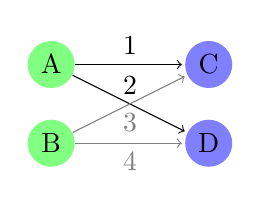
\begin{tikzpicture}[shorten >=1pt, ->, draw=black!50, node distance=\layersep]
      \tikzstyle{every pin edge}=[<-, shorten <=1pt]
      \tikzstyle{neuron}=[circle, fill=black!25, minimum size=17pt, inner sep=0pt]
      \tikzstyle{input neuron}=[neuron, fill=green!50];
      \tikzstyle{output neuron}=[neuron, fill=red!50];
      \tikzstyle{hidden neuron}=[neuron, fill=blue!50];
      \tikzstyle{annot} = [text width=4em, text centered]
      
      \node[input neuron] (A) at (0, 0) {A};
      \node[input neuron] (B) at (0, -1) {B};
      \node[hidden neuron] (C) at (2, 0) {C};
      \node[hidden neuron] (D) at (2, -1) {D};
      
      \path (A) edge [color=black] node [above] {1} (C);
      \path (A) edge [color=black] node [above] {2} (D);
      \path (B) edge [color=gray] node [below] {3} (C);
      \path (B) edge [color=gray] node [below] {4} (D);
  \end{tikzpicture}
  ~~~~~~~~
  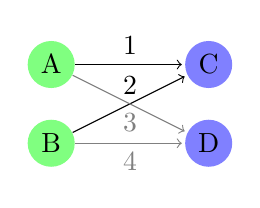
\begin{tikzpicture}[shorten >=1pt, ->, draw=black!50, node distance=\layersep]
      \tikzstyle{every pin edge}=[<-, shorten <=1pt]
      \tikzstyle{neuron}=[circle, fill=black!25, minimum size=17pt, inner sep=0pt]
      \tikzstyle{input neuron}=[neuron, fill=green!50];
      \tikzstyle{output neuron}=[neuron, fill=red!50];
      \tikzstyle{hidden neuron}=[neuron, fill=blue!50];
      \tikzstyle{annot} = [text width=4em, text centered]
      
      \node[input neuron] (A) at (0, 0) {A};
      \node[input neuron] (B) at (0, -1) {B};
      \node[hidden neuron] (C) at (2, 0) {C};
      \node[hidden neuron] (D) at (2, -1) {D};
      
      \path (A) edge [color=black] node [above] {1} (C);
      \path (B) edge [color=black] node [above] {2} (C);
      \path (A) edge [color=gray] node [below] {3} (D);
      \path (B) edge [color=gray] node [below] {4} (D);
  \end{tikzpicture}
  \caption{Examples of the weight assignments in the experiments}
  \label{differentresults}
 \end{figure}
 
 \subsection{From each input node \ldots}
  
  For the first data extraction, we got the results as in Figure \ref{firstlast}. Note that the least and most variance in randomness are respectively the first and last result when sorting the results, and therefore they are called ``first'' and ``last'' in the figure. As we can see, with more than one hidden node the highest error is achieved with the scheme with the least variance. However, this does not hold true for the experiment with only one hidden node. Also, the lowest error is achieved on a scheme which does not seem to correspond with having a high variance or not. An early conclusion therefore is that having as much variance as possible in the weights does not necessarily give the lowest error.\\
  
  \begin{figure}[h!]
  	\begin{verbatim}
One hidden node
first,   AAAAA,              103.4516
last,    ABCDE,              108.8348
highest, ABBBB,              113.9604
lowest,  AAABC,              103.4155

Two hidden nodes
first,   AAAAAAAAA,          119.2281
last,    ABCDEFGHI,          73.94541
highest, AAAAAAAAA,          119.2281
lowest,  ABBBCDDDE,          60.62256

Three hidden nodes
first,   AAAAAAAAAAAAA,      142.6884
last,    ABCDEFGHIJKLM,      19.35041
highest, AAAAAAAAAAAAA,      142.6884
lowest,  AABCDDDEEEFFF,      8.865258

Four hidden nodes
first,   AAAAAAAAAAAAAAAAA,  133.1499
last,    ABCDEFGHIJKLMNOPQ,  7.661870
highest, AAAAAAAAAAAAAAAAA,  133.1499
lowest,  AABBBBBBBCCCDEEFF,  0.198013
  	\end{verbatim}
  	\caption{Specific values from the results in the first experiment.}
  	\label{firstlast}
  \end{figure}
  For the second data extraction, the results are as in Figure \ref{varianceaverage}. Here the first number indicates the amount of different weights in the scheme; $0$ indicates that all weights are the same, $1$ indicates that there are two different weights, etc. The numbers behind it are the average errorsums of all schemes which have the amount of different weights as according to the first number. This means that the first row, starting with the $0$, is the average over the four schemes where all weights were the same, one for each experiment (where the one value of each experiment is already the average over the $91$ seeds on which the experiment was run). As we can see in this figure, on average the higher the variance in the weights, the lower the error rate is.
  
  \begin{figure}[h!]
  	\begin{verbatim}
0: 124.6295    9: 8.981157
1: 41.70797    10: 8.717536
2: 26.60600    11: 8.471507
3: 18.76652    12: 8.384696
4: 14.46136    13: 8.295702
5: 12.11053    14: 8.166788
6: 10.78785    15: 7.918954
7: 9.969623    16: 7.661870
8: 9.345573
  	\end{verbatim}
  	\caption{Average error over each variance in weights in the first experiment, with the first number being the amount of different weights in a scheme and the second number being the average error.}
  	\label{varianceaverage}
  \end{figure}

  \subsection{\ldots~to each hidden node}
  In comparison to these initial results, we ran the experiment again with another method of interpreting the weight schemes, as explained at the beginning of this section. The corresponding results of this second experiment are shown in Figures \ref{firstlastreverse} and \ref{variancereverse}. As can be seen, the specific extracted values are all higher than their counterparts in the first experiment, with the exception of some values in the part of the experiment where a hidden layer of three nodes is used. The difference is not that big however, except for the error value of the last scheme with four hidden nodes, where the result from the second experiment is $3138\%$ higher!\\
  Besides this, the average error over he variance also shows a little fluctuation compared to the first experiment, however more surprising is that the trend shown in the first experiment is not completely present in the second experiment. The average error does in general go down when more variance in the weight scheme is introduced, but not all average errors are consistently lower than the ``previous" ones (with lower variance), as the average error of variance 13 is slightly higher than that of 12, and the average error of variance 15 is noticably higher than those of the 5 previous variances.
  
  \begin{figure}[h!]
  	\begin{verbatim}
One hidden node
first,   AAAAA,              107.7259
last,    ABCDE,              115.1607
highest, ABCDE,              115.1607
lowest,  AABBC,              104.9102

Two hidden nodes
first,   AAAAAAAAA,          124.6325
last,    ABCDEFGHI,          73.14062
highest, AAAAAAAAA,          124.6325
lowest,  ABCCDDDEF,          61.45848

Three hidden nodes
first,   AAAAAAAAAAAAA,      139.5990
last,    ABCDEFGHIJKLM,      15.67902
highest, AAAAAAAAAAAAA,      139.5990
lowest,  ABBBCCDEFFFGG,      8.880461

Four hidden nodes
first,   AAAAAAAAAAAAAAAAA,  134.6954
last,    ABCDEFGHIJKLMNOPQ,  7.691363
highest, AAAAAAAAAAAAAAAAA,  134.6954
lowest,  AAAAABBBCDDDEEEFF,  6.213909
  	\end{verbatim}
  	\caption{Specific values from the results in the second experiment.}
  	\label{firstlastreverse}
  \end{figure}
  
  \begin{figure}[h!]
  	\begin{verbatim}
0: 126.6632    9: 8.933152
1: 39.34963    10: 8.692506
2: 24.48846    11: 8.569032
3: 17.61451    12: 8.354593
4: 13.84969    13: 8.355490
5: 11.77741    14: 8.204631
6: 10.56131    15: 8.840239
7: 9.806410    16: 7.691363
8: 9.308938
  	\end{verbatim}
  	\caption{Average error over each variance in weights in the second experiment, with the first number being the amount of different weights in a scheme and the second number being the average error.}
  	\label{variancereverse}
  \end{figure}
  
  \subsection{Pull it together!}
  In the third experiment, a new method called ``nudging" is tested. This method essentially tries to enforce the weight scheme throughout the experiment, rather than only at the start. So for any edge x which has been assigned letter y according to the weight scheme, if there is another edge z which has been assigned the same letter y according to the weight scheme, the weights of those edges will be ``nudged" to each other, and to the weight of each other edge which has been assigned the letter y. If we have edges $a_1$, $a_2$, and $b_1$ with weight scheme ABC, then $a_1$ has been assigned A, $a_2$ has been assigned B, and $b_1$ has been assigned C. \\
  The nudging consists of taking the average of the weights of all edges assigned the same letter, and then to assign to each edge its weight subtracted by half the difference between said weight and the average of the weights. So for weight $w_1$ and average $W$ over weights $w_1, w_2, \ldots, w_n$, the new weight is calculated as follows: 
  $${w_1}^{n + 1} = {w_1}^n - \frac{({w_1}^n - W)}{2}$$
  This nudging is then applied to all weights every 500 epochs, whereas the frequency of applying the nudging is a trade off between the effect being notably present and between the nudging not overly limiting the amount of change a weight can make through the experiment. This means that with a higher frequency the weights may not adapt sufficiently to the data, and with a lower frequency the weights may not be similar enough to be properly nudged to each other.\\
  As the results in appendix \ref{nudgeappendix} point out, the effect of the nudging is desastrous to say in the least, compared to previous results. Whereas the the previous highest summed error recorded was slightly more than $142$, none of the summed errors in this experiment go below $178$. The summed errors for each of the variances, which showed improvement in the previous experiments when more weights were initialised on different values, also show no noteworthy improvement, or even none at all. Do note that this experiment has been run twice with the exact same results, due to our utter disbelief that these results can be correct.
  
 \section{Conclusion}
 \label{conclusion}
  A Deep Learning network is a collection of entities and relations, called nodes and edges, through which certain input is propagated to give a certain output. This network can then be trained by backward propagation, using the error which is the result of comparing the calculated output with the expected output, which updates the weights of the edges. This way, the forward propagation will most likely yield different results, and this process can then be repeated until an acceptable error margin is reached. We implemented a small version of such a network to decide on the possibility and usability of a smaller network for certain tasks.\\
	 After seeming initial failure of performing experiments based on the code initialising the same weight to every edge in the network, the hypothesis was that the amount of randomness in the initialisation of the weights, with ``more random'' meaning that less weights have the same value, influenced the accuracy of the network. To test this, the network was trained and tested on the XOR-problem multiple times, each with a different fixed seed to ensure controlled randomness on a large enough test group, with different amounts of weights having the same initial value. As we can see in Section \ref{results}, at the very least this hypothesis holds true, and four additional conclusions can be drawn.\\
	 The first additional conclusion is that ``more randomness'' does not always ensure better results. As seen in Figure \ref{firstlast}, the weight scheme with the lowest average error does in no case coincide with the ``most random'' weight scheme. On the other hand, ``less randomness'' does ensure worse results, as for the experiments with more than one hidden node the weight scheme with the highest error appears to be the same as the weight scheme with the least randomness. The outlier is the experiment with only one hidden node, plus bias node, where the weight scheme with all weights on the same initial value performs almost as well as the weight scheme with the lowest error, and the weight scheme with the most randomness is somewhere in between the lowest and highest error values.\\
	 The second additional conclusion is that, based on Figure \ref{varianceaverage}, with more randomness in the weight scheme the error is lower on average. While one may argue that the weight schemes AAAAB and ABBBB are by no means comparable, the results show that having as much randomness as possible in general will result in a lower error. The average error does not appear to lower at a constant rate, but between each variance in randomness it \emph{is} lower. Using these two additional conclusions, this means that while having as much randomness as possible in the weight scheme may not produce the best results for a specific problem, in general more randomness does lead to better results.\\
	 The third addition conclusion is, as shown in the second experiment, that the manner of interpreting the weight scheme can also impact the performance of the network. While the difference may be minimal on average, comparison between both Figures \ref{firstlast} and \ref{firstlastreverse} and Figures \ref{varianceaverage} and \ref{variancereverse} shows that the first experiment had lower errors in general. Therefore, when using weight schemes to control the assignment of the randomly generated weights to the edges of the network, it is recommended to assign all the edges from each node in the previous layer, as opposed to t\'o each node in the next layer.\\
	 Lastly, the fourth additional conclusion is that the process of ``nudging", which lightly enforces a scheme throughout the course of the program at certain intervals, is not recommended for use. The results achieved in the experiment, which can be seen in appendix \ref{nudgeappendix}, show that usage of this process ensures an incredibly high error rate and that it is therefore of no use to any application of Deep Learning.\\
	 For future work, research can be done regarding the influences of the specific patterns weight schemes: for example, if having the same initial weight on the bias nodes and the other weights being completely random would increase performance, or if when each weight on each layer has the same initial value, but that differs between layers, the performance improves, etc. Also, research can be done with multiple hidden layers to see if the same conclusions hold for that case as well. Lastly, more complex problems with possibly more output nodes may lead to different conclusions on this research as well.
 
\begin{thebibliography}{XX}

\bibitem{DeepLearning}
Yann LeCun, Yoshua Bengio, and Geoffrey Hinton. ``Deep learning." Nature, 521, 7553, 2015, pp. 436–444.

\bibitem{AlphaGo}
 David Silver, Aja Huang, Chris J. Maddison, Arthur Guez, Laurent Sifre, George van den Driessche, Julian Schrittwieser, Ioannis Antonoglou, Veda Panneershelvam, Marc Lanctot, Sander Dieleman, Dominik Grewe, John Nham, Nal Kalchbrenner, Ilya Sutskever, Timothy Lillicrap, Madeleine Leach, Koray Kavukcuoglu, Thore Graepel, Demis Hassabis. “Mastering the Game of Go with Deep Neural Networks and Tree Search.” Nature, vol. 529, no. 7587, 2016, pp. 484–489.
 
\bibitem{AlphaGoZero}
 David Silver, Julian Schrittwieser, Karen Simonyan, Ioannis Antonoglou, Aja Huang, Arthur Guez, Thomas Hubert, Lucas Baker, Matthew Lai, Adrian Bolton, Yutian Chen, Timothy Lillicrap, Fan Hui, Laurent Sifre, George van den Driessche, Thore Graepel, Demis Hassabis. “Mastering the Game of Go without Human Knowledge.” Nature, vol. 550, no. 7676, 2017, pp. 354–359. 
 
\bibitem{StarCraft}
Oriol Vinyals, Timo Ewalds, Sergey Bartunov, Petko Georgiev, Alexander Sasha Vezhnevets, Michelle Yeo, Alireza Makhzani, Heinrich Küttler, John Agapiou, Julian Schrittwieser, Stephen Gaffney, Stig Petersen, Karen Simonyan, Tom Schaul, Hado van Hasselt, David Silver, Timothy Lillicrap, Kevin Calderone, Paul Keet, Anthony Brunasso, David Lawrence, Anders Ekermo, Jacob Repp, Rodney Tsing. ``StarCraft II: A New Challenge for
Reinforcement Learning.", arXiv:1708.04782.

\bibitem{NotesBack}
Peter Sadowski. ``Notes on backpropagation." \url{https://www.ics.uci.edu/~pjsadows/notes.pdf}, 2016.

\end{thebibliography}

\newpage

\appendix
\section*{Appendices}
\addcontentsline{toc}{section}{Appendices}
\renewcommand{\thesubsection}{\Alph{subsection}}

\subsection{Results of the nudging experiment}
\label{nudgeappendix}

\subsubsection{Extremes}
\FloatBarrier

Each figure in this subsection shows the extreme values in the experiment with nudging. The values are the value of the scheme where all weights are the same, the value of the scheme where all values are different, the value which is the highest and its corresponding scheme, and the value which is the lowest and its corresponding scheme. The caption on each figure shows at which epoch the results were recorded.

\FloatBarrier

\begin{figure}[!ht]
 \begin{verbatim}
first:   AAAAAAAAAAAAAAA, 182.1243
last:    ABCDEFGHIJKLMNO, 182.2900
highest: ABBBBBBCCDEFFGG, 183.8708
lowest:  AAAAABBCDDEFGHH, 180.5045
 \end{verbatim}
 \vspace{-20pt} 
 \caption{The extremes of epoch $1000$.}
\end{figure}


\begin{figure}[!ht]
 \begin{verbatim}
first:   AAAAAAAAAAAAAAA, 181.9728
last:    ABCDEFGHIJKLMNO, 181.9717
highest: ABCCDDDEFFFFGGG, 182.6064
lowest:  AAABCDEEFGHHHHI, 179.8012
 \end{verbatim}
 \vspace{-20pt} 
 \caption{The extremes of epoch $2000$.}
\end{figure}


\begin{figure}[!ht]
 \begin{verbatim}
first:   AAAAAAAAAAAAAAA, 182.1200
last:    ABCDEFGHIJKLMNO, 180.9563
highest: ABCDDDDEFGGGGGG, 184.5941
lowest:  ABCCDDDDDEFGHII, 177.2216
 \end{verbatim}
 \vspace{-20pt} 
 \caption{The extremes of epoch $3000$.}
\end{figure}


\begin{figure}[!ht]
 \begin{verbatim}
first:   AAAAAAAAAAAAAAA, 182.0176
last:    ABCDEFGHIJKLMNO, 181.4683
highest: ABCDDDEEEFGGHIJ, 183.6219
lowest:  ABCDEFFGGHHHHII, 178.3634
 \end{verbatim}
 \vspace{-20pt} 
 \caption{The extremes of epoch $4000$.}
\end{figure}

\begin{figure}[!ht]
 \begin{verbatim}
first:   AAAAAAAAAAAAAAA, 182.0010
last:    ABCDEFGHIJKLMNO, 181.1900
highest: ABCCDDEEFFFGGHH, 183.7443
lowest:  ABBBBCCCDDEEEFG, 178.5798
 \end{verbatim}
 \vspace{-20pt} 
 \caption{The extremes of epoch $5000$.}
\end{figure}


\begin{figure}[!ht]
 \begin{verbatim}
first:   AAAAAAAAAAAAAAA, 181.9981
last:    ABCDEFGHIJKLMNO, 181.2439
highest: ABCDDDDEFGHIIJK, 183.2607
lowest:  ABCCDDDDDDDDEEE, 178.8257
 \end{verbatim}
 \vspace{-20pt} 
 \caption{The extremes of epoch $6000$.}
\end{figure}


\begin{figure}[!ht]
 \begin{verbatim}
first:   AAAAAAAAAAAAAAA, 181.9867
last:    ABCDEFGHIJKLMNO, 180.2469
highest: ABCDDEEEFGGGHIJ, 184.2835
lowest:  AAABCDEEEFGGGGG, 177.3950
 \end{verbatim}
 \vspace{-20pt} 
 \caption{The extremes of epoch $7000$.}
\end{figure}


\begin{figure}[!ht]
 \begin{verbatim}
first:   AAAAAAAAAAAAAAA, 181.9994
last:    ABCDEFGHIJKLMNO, 181.6152
highest: ABCDDEEEFGGGGHH, 183.4335
lowest:  ABCCDDDDDEFFFGH, 178.3849
 \end{verbatim}
 \vspace{-20pt} 
 \caption{The extremes of epoch $8000$.}
\end{figure}


\begin{figure}[!ht]
 \begin{verbatim}
first:   AAAAAAAAAAAAAAA, 182.0009
last:    ABCDEFGHIJKLMNO, 180.4394
highest: ABCDDDEEEFGGHHH, 184.2179
lowest:  ABCCDDEFGHHHHIJ, 178.4969
 \end{verbatim}
 \vspace{-20pt} 
 \caption{The extremes of epoch $9000$.}
\end{figure}

\begin{figure}[!ht]
 \begin{verbatim}
first:   AAAAAAAAAAAAAAA, 181.9992
last:    ABCDEFGHIJKLMNO, 181.1662
highest: ABCDDDDEFGHHHIJ, 184.0517
lowest:  ABCCDEEEEFGGGHH, 178.5642
 \end{verbatim}
 \vspace{-20pt} 
 \caption{The extremes of epoch $10000$.}
\end{figure}

\begin{figure}[!ht]
 \begin{verbatim}
first:   AAAAAAAAAAAAAAA, 182.0000
last:    ABCDEFGHIJKLMNO, 181.0202
highest: ABCDDDDDEFGHHHH, 182.9620
lowest:  ABCCDDEFGHHIIIJ, 178.8305
 \end{verbatim}
 \vspace{-20pt} 
 \caption{The extremes of epoch $11000$.}
\end{figure}


\begin{figure}[!ht]
 \begin{verbatim}
first:   AAAAAAAAAAAAAAA, 182.0000
last:    ABCDEFGHIJKLMNO, 180.4485
highest: ABCDDDDEFGHHIJJ, 183.9073
lowest:  ABCCDEEEEFGHHHH, 178.5546

 \end{verbatim}
 \vspace{-20pt} 
 \caption{The extremes of epoch $12000$.}
\end{figure}


\begin{figure}[!ht]
 \begin{verbatim}
first:   AAAAAAAAAAAAAAA, 182.0000
last:    ABCDEFGHIJKLMNO, 181.3162
highest: ABCDDDDEFGGGHHH, 183.1856
lowest:  ABCCDDEFGHHHHII, 179.2354
 \end{verbatim}
 \vspace{-20pt} 
 \caption{The extremes of epoch $13000$.}
\end{figure}

\begin{figure}[!ht]
 \begin{verbatim}
first:   AAAAAAAAAAAAAAA, 182.0000
last:    ABCDEFGHIJKLMNO, 181.3967
highest: ABCDDDDDEFFFFFG, 183.3238
lowest:  ABCCDDDDDEFFGGG, 178.9348
 \end{verbatim}
 \vspace{-20pt} 
 \caption{The extremes of epoch $14000$.}
\end{figure}


\begin{figure}[!ht]
 \begin{verbatim}
first:   AAAAAAAAAAAAAAA, 182.0000
last:    ABCDEFGHIJKLMNO, 181.5964
highest: ABCDDDDEFGGGHII, 183.4648
lowest:  ABCCDDEEEEEFGHI, 178.8923
 \end{verbatim}
 \vspace{-20pt} 
 \caption{The extremes of epoch $15000$.}
\end{figure}


\begin{figure}[!ht]
 \begin{verbatim}
first:   AAAAAAAAAAAAAAA, 182.0000
last:    ABCDEFGHIJKLMNO, 181.1856
highest: AABCCCCDEFGGHHH, 183.4760
lowest:  ABBCDEFGGHHHIJK, 179.2380
 \end{verbatim}
 \vspace{-20pt} 
 \caption{The extremes of epoch $16000$.}
\end{figure}


\begin{figure}[!ht]
 \begin{verbatim}
first:   AAAAAAAAAAAAAAA, 182.0000
last:    ABCDEFGHIJKLMNO, 181.7291
highest: ABCDDDEEFFFFFFF, 183.2565
lowest:  ABCCDDEEEEEFFFG, 179.2174
 \end{verbatim}
 \vspace{-20pt} 
 \caption{The extremes of epoch $17000$.}
\end{figure}


\begin{figure}[!ht]
 \begin{verbatim}
first:   AAAAAAAAAAAAAAA, 182.0000
last:    ABCDEFGHIJKLMNO, 181.6613
highest: ABCDDDDDDEEFGHI, 183.0773
lowest:  AABBCCDDDDEFFGG, 178.7635
 \end{verbatim}
 \vspace{-20pt} 
 \caption{The extremes of epoch $18000$.}
\end{figure}

\begin{figure}[!ht]
 \begin{verbatim}
first:   AAAAAAAAAAAAAAA, 182.0000
last:    ABCDEFGHIJKLMNO, 180.9126
highest: ABCDDDEEFFFFFFF, 183.2365
lowest:  ABCCDDDDDEEEEFF, 179.2136
 \end{verbatim}
 \vspace{-20pt} 
 \caption{The extremes of epoch $19000$.}
\end{figure}


\begin{figure}[!ht]
 \begin{verbatim}
first:   AAAAAAAAAAAAAAA, 182.0000
last:    ABCDEFGHIJKLMNO, 180.5785
highest: ABCDDDDDEFFFGGH, 183.5244
lowest:  ABCDEEFGHIIIIJK, 178.7214
 \end{verbatim}
 \vspace{-20pt} 
 \caption{The extremes of epoch $20000$.}
\end{figure}

\FloatBarrier

\subsubsection{Variances}

Each figure in this subsection shows the average error over each variance in weights in the experiment with nudging, with the first number being the amount of weights in each scheme which are different to each other and the second number being the average error. The caption on each figure shows at which epoch the results were recorded.

\FloatBarrier

\begin{figure}[!ht]
 \begin{verbatim}
0: 181.9992    8:  181.6769
1: 181.9928    9:  181.6374
2: 181.9216    10: 181.5689
3: 181.8861    11: 181.4702
4: 181.8371    12: 181.3549
5: 181.8039    13: 181.1953
6: 181.7629    14: 181.1662
7: 181.7247
 \end{verbatim}
 \vspace{-20pt} 
 \caption{The variances of epoch $10000$.}
\end{figure}

\begin{figure}[!ht]
 \begin{verbatim}
0: 182.1243    8:  182.0389
1: 182.0084    9:  182.0578
2: 181.9534    10: 182.0765
3: 181.9312    11: 182.1074
4: 181.9358    12: 182.1455
5: 181.9551    13: 182.1811
6: 181.9744    14: 182.2900
7: 182.0009
 \end{verbatim}
 \vspace{-20pt} 
 \caption{The variances of epoch $1000$.}
\end{figure}

\begin{figure}[!ht]
 \begin{verbatim}
0: 181.9999    8:  181.6389
1: 181.9871    9:  181.5915
2: 181.9497    10: 181.5441
3: 181.9036    11: 181.4689
4: 181.8350    12: 181.4115
5: 181.7805    13: 181.1805
6: 181.7339    14: 181.0202
7: 181.6810
 \end{verbatim}
 \vspace{-20pt} 
 \caption{The variances of epoch $11000$.}
\end{figure}

\begin{figure}[!ht]
 \begin{verbatim}
0: 182.0000    8:  181.6596
1: 181.9768    9:  181.6042
2: 181.9430    10: 181.5588
3: 181.9107    11: 181.4699
4: 181.8594    12: 181.4723
5: 181.8010    13: 181.2092
6: 181.7588    14: 180.4485
7: 181.7090
 \end{verbatim}
 \vspace{-20pt} 
 \caption{The variances of epoch $12000$.}
\end{figure}

\begin{figure}[!ht]
 \begin{verbatim}
0: 182.0000    8:  181.6786
1: 181.9947    9:  181.6391
2: 181.9534    10: 181.5687
3: 181.9093    11: 181.5162
4: 181.8639    12: 181.3814
5: 181.8140    13: 181.1223
6: 181.7649    14: 181.3162
7: 181.7222
 \end{verbatim}
 \vspace{-20pt} 
 \caption{The variances of epoch $13000$.}
\end{figure}


\begin{figure}[!ht]
 \begin{verbatim}
0: 182.0000    8:  181.6938
1: 181.9960    9:  181.6550
2: 181.9674    10: 181.6065
3: 181.9198    11: 181.4924
4: 181.8780    12: 181.4495
5: 181.8301    13: 181.2579
6: 181.7886    14: 181.3967
7: 181.7400
 \end{verbatim}
 \vspace{-20pt} 
 \caption{The variances of epoch $14000$.}
\end{figure}

\begin{figure}[!ht]
 \begin{verbatim}
0: 182.0000    8:  181.6645
1: 181.9614    9:  181.6152
2: 181.9564    10: 181.5439
3: 181.9190    11: 181.4648
4: 181.8708    12: 181.3838
5: 181.8186    13: 181.1860
6: 181.7715    14: 181.5964
7: 181.7137
 \end{verbatim}
 \vspace{-20pt} 
 \caption{The variances of epoch $15000$.}
\end{figure}

\begin{figure}[!ht]
 \begin{verbatim}
0: 182.0000    8:  181.6766
1: 181.9863    9:  181.6131
2: 181.9724    10: 181.5608
3: 181.9248    11: 181.4578
4: 181.8845    12: 181.3177
5: 181.8300    13: 181.3309
6: 181.7794    14: 181.1856
7: 181.7309
 \end{verbatim}
 \vspace{-20pt} 
 \caption{The variances of epoch $16000$.}
\end{figure}

\begin{figure}[!ht]
 \begin{verbatim}
0: 182.0000    8:  181.6841
1: 181.9976    9:  181.6265
2: 181.9646    10: 181.5758
3: 181.9331    11: 181.5193
4: 181.8871    12: 181.4329
5: 181.8417    13: 181.2052
6: 181.7882    14: 181.7291
7: 181.7322
 \end{verbatim}
 \vspace{-20pt} 
 \caption{The variances of epoch $17000$.}
\end{figure}

\begin{figure}[!ht]
 \begin{verbatim}
0: 182.0000    8:  181.691
1: 181.9891    9:  181.6328
2: 181.9780    10: 181.5743
3: 181.9423    11: 181.4830
4: 181.8924    12: 181.3174
5: 181.8403    13: 181.3544
6: 181.7898    14: 181.6613
7: 181.7447
 \end{verbatim}
 \vspace{-20pt} 
 \caption{The variances of epoch $18000$.}
\end{figure}

\begin{figure}[!ht]
 \begin{verbatim}
0: 182.0000    8:  181.6619
1: 181.9912    9:  181.6013
2: 181.9669    10: 181.5237
3: 181.9321    11: 181.4631
4: 181.8904    12: 181.3789
5: 181.8374    13: 181.2554
6: 181.7868    14: 180.9126
7: 181.7281
 \end{verbatim}
 \vspace{-20pt} 
 \caption{The variances of epoch $19000$.}
\end{figure}

\begin{figure}[!ht]
 \begin{verbatim}
0: 182.0000    8:  181.6843
1: 181.9991    9:  181.6186
2: 181.9749    10: 181.5539
3: 181.9457    11: 181.4428
4: 181.8969    12: 181.3317
5: 181.8457    13: 181.1582
6: 181.8007    14: 180.5785
7: 181.7470
 \end{verbatim}
 \vspace{-20pt} 
 \caption{The variances of epoch $20000$.}
\end{figure}

\begin{figure}[!ht]
 \begin{verbatim}
0: 181.9728    8:  181.7606
1: 181.9765    9:  181.7602
2: 181.9299    10: 181.7939
3: 181.8812    11: 181.8147
4: 181.8371    12: 181.8580
5: 181.7989    13: 181.9300
6: 181.7738    14: 181.9717
7: 181.7594
 \end{verbatim}
 \vspace{-20pt} 
 \caption{The variances of epoch $2000$.}
\end{figure}

\begin{figure}[!ht]
 \begin{verbatim}
0: 182.1200    8:  181.2167
1: 181.9573    9:  181.1417
2: 181.7086    10: 181.0711
3: 181.5432    11: 180.9470
4: 181.4437    12: 180.9782
5: 181.3606    13: 180.8150
6: 181.3068    14: 180.9563
7: 181.2616
 \end{verbatim}
 \vspace{-20pt} 
 \caption{The variances of epoch $3000$.}
\end{figure}

\begin{figure}[!ht]
 \begin{verbatim}
0: 182.0176    8:  181.6627
1: 181.9814    9:  181.6202
2: 181.8715    10: 181.5394
3: 181.8180    11: 181.4519
4: 181.7717    12: 181.3427
5: 181.7437    13: 181.1746
6: 181.7311    14: 181.4683
7: 181.6992
 \end{verbatim}
 \vspace{-20pt} 
 \caption{The variances of epoch $4000$.}
\end{figure}

\begin{figure}[!ht]
 \begin{verbatim}
0: 182.0010    8:  181.7700
1: 181.9765    9:  181.7441
2: 181.9223    10: 181.6996
3: 181.8507    11: 181.6379
4: 181.7994    12: 181.5468
5: 181.7772    13: 181.4097
6: 181.7696    14: 181.1900
7: 181.7758
 \end{verbatim}
 \vspace{-20pt} 
 \caption{The variances of epoch $5000$.}
\end{figure}

\begin{figure}[!ht]
 \begin{verbatim}
0: 181.9981    8:  181.7410
1: 181.9699    9:  181.7109
2: 181.9258    10: 181.6708
3: 181.8658    11: 181.6069
4: 181.8187    12: 181.5378
5: 181.7936    13: 181.3748
6: 181.7746    14: 181.2439
7: 181.7556
 \end{verbatim}
 \vspace{-20pt} 
 \caption{The variances of epoch $6000$.}
\end{figure}

\begin{figure}[!ht]
 \begin{verbatim}
0: 181.9867    8:  181.5815
1: 181.9838    9:  181.5191
2: 181.9019    10: 181.4168
3: 181.8098    11: 181.2640
4: 181.7293    12: 181.1311
5: 181.6903    13: 180.7969
6: 181.6576    14: 180.2469
7: 181.6222
 \end{verbatim}
 \vspace{-20pt} 
 \caption{The variances of epoch $7000$.}
\end{figure}

\begin{figure}[!ht]
 \begin{verbatim}
0: 181.9994    8:  181.6717
1: 181.9800    9:  181.6024
2: 181.9263    10: 181.5086
3: 181.8872    11: 181.4339
4: 181.8285    12: 181.2425
5: 181.7892    13: 181.3121
6: 181.7626    14: 181.6152
7: 181.7248
 \end{verbatim}
 \vspace{-20pt} 
 \caption{The variances of epoch $8000$.}
\end{figure}

\begin{figure}[!ht]
 \begin{verbatim}
0: 182.0009    8:  181.6589
1: 181.9888    9:  181.6027
2: 181.9434    10: 181.5261
3: 181.8925    11: 181.4399
4: 181.8356    12: 181.2598
5: 181.7914    13: 181.3152
6: 181.7448    14: 180.4393
7: 181.7113
 \end{verbatim}
 \vspace{-20pt} 
 \caption{The variances of epoch $9000$.}
\end{figure}
 
\end{document}
